\documentclass[tikz, margin=5mm]{standalone}

\usetikzlibrary{arrows.meta, chains, positioning}

\begin{document}
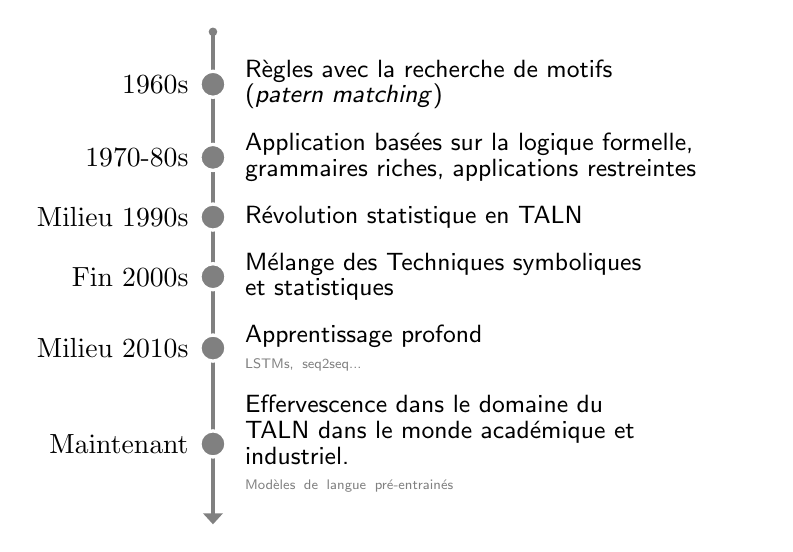
\begin{tikzpicture}[
    node distance = 1mm and 3mm,
    start chain = A going below,
    dot/.style = {circle, draw=white, very thick, fill=gray, minimum size=3mm},
    box/.style = {rectangle, text width=62mm, inner xsep=4mm, inner ysep=1mm, font=\sffamily\small\linespread{0.84}\selectfont, on chain},
]
    \begin{scope}[every node/.append style={box}]
        % Définir ici un nœud par évènement
        \node { Règles avec la recherche de motifs \\
                (\emph{patern matching})};
        \node { Application basées sur la logique formelle, grammaires riches, applications restreintes};
        \node { Révolution statistique en TALN };
        \node { Mélange des Techniques symboliques \\
                et statistiques };
        \node { Apprentissage profond \\
                \textcolor{gray}{\tiny LSTMs, seq2seq...} };
        \node { Effervescence dans le domaine du \\
                TALN dans le monde académique et \\
                industriel.  \\
                \textcolor{gray}{\tiny Modèles de langue pré-entrainés} };
    \end{scope}
    \draw[very thick, gray, {Triangle[length=4pt]}-{Circle[length=3pt]}, shorten <=-3mm, shorten >=-3mm] (A-6.south west) -- (A-1.north west);
    % Définir ci-dessous les dates des évènements, dans l'ordre.
    \foreach \i [ count=\j] in {1960s, 1970-80s, Milieu 1990s, Fin 2000s, Milieu 2010s, Maintenant}
        \node[dot,label=left:\i] at (A-\j.west) {};
\end{tikzpicture}
\end{document}